\begin{table*}[t]
	\begin{tabular}{|l||l|c|c|c|c|c|c|}
		\hline
		Resource
		& Purpose 	& \#Cat & \#Ref/ & \#Refs
		& \multicolumn{2}{c|}{Constraints on} 
		& WordNet  \\
		& & & object			
		& 			
		& language 	& images 
		& IDs?\\
		\hline \hline
		\refcoco 	& REG,REC
					& 80 & 3 & 50k
					& -				
					& $\geq$2 objs  
					& \xmark \\
					&
					& & & 
					& 
					& of same cat
					& \\
		\refcocop 	& REG,REC
					& 80 & 3 & 50k
					& + 			
					& $\geq$2 objs  
					& \xmark \\	
					&
					& & & 
					& 
					& of same cat
					& \\
		\flickr 	& Phrase localization
					& ?	& & 
					& -- 
					& & \xmark \\
					& Caption generation
					& & & &  \\
		\vgenome 	& Scene understanding 
					& 80k & & 
					& & & \cmark\\
					& Phrase localization
					& & & &  \\
		\hline
	\end{tabular}
	\caption{\label{tab:summary_resources} Overview of V\&L benchmarks for taks related to reference. Cat: Categories; Ref: Reference; REG and REC: Referring expression generation and comprehension, respectively.}
\end{table*}

\begin{table*}[t]
	\begin{center}
	\begin{tabular}{|l|c|c|c|c|}
		\hline
		Resource & \multicolumn{3}{c|}{Provides (more or less directly)}\\
		 		 & R1: Root-level & R2: Entry-level & R4: Coordinates  \\
		\hline \hline
		\refcoco 	& \xmark & \xmark & \cmark \\
		\refcocop 	& \xmark & \xmark & \cmark \\
		\flickr 	& \xmark & (\cmark) & \cmark \\
		\vgenome 	& \xmark & \cmark 	& \cmark \\
		\hline 		
	\end{tabular}
	\caption{\label{tab:summary_resources} BLABLA overview of resources and their shortcomings wrt object naming. REG and REC: Referring expression generation and comprehension, respectively.}
	\end{center}
\end{table*}

\subsection{Linguistic Resources, Computer Vision Resources}
\paragraph{WordNet}
WordNet \cite{fellbaum1998wordnet} blabla. 

\paragraph{Methods: Object Detectors, Image Classifiers} \cs{Do we need that? I would say no.}

\paragraph{ImageNet and ILSVRC}


\paragraph{MS COCO} \cite{mscoco}
MS COCO is an object recognition dataset of images of natural scenes of $91$~common object categories (e.g.,~\cat{dog, pizza, chair}). 
Multiple datasets for vision \& language tasks have been built on top of COCO, such as the referring expressions datasets \refcoco and \refcocop which we will discuss below, and \textsl{COCO Captions} \cite{chen2015cococaptions}.  
The latter provides five captions for each of  $300k$~images, spanning $80$~of the COCO categories.  
However, the COCO region-level (object) annotations are not linked to the captions.
\subsection{V\ \&\ L Resources}

\paragraph{\refcoco and \refcocop \cite{Yu2016}}~\\ 
Both datasets are extensions of \referit\cite{Kazemzadeh2014}, a large-scale collection of referring expressions (RE) for natural objects in real-world images, and are built on top of the MS COCO image collection \cite{mscoco}. 

The REs were collected via crowdsourcing in a two-player game, which was designed to obtain REs uniquely referring to the target objects in an image. 
Specifically, a director and a matcher are presented with an image, and the director produces a RE for an outlined target object in the image. 
The matcher must click on the object he thinks the RE refers to. 
If the matcher's prediction is correct, the RE is considered valid. 
For more details on the datasets see \cite{Yu2016}.

Finally, \referit is based on the SAIAPR image collection \cite{Grubinger2006} (20k images;99.5k image regions;120K REs), and captures not only REs for objects ("things") but also for scene categories (e.g.,{\refexp{grass, road}) (see also \cite{hu2015,mao2016generation}). 
The task of scene detection is beyond the focus of our study regarding object naming, we therefore will not discuss this dataset further.

\paragraph{Flickr30k Entities}~\\
The \flickr dataset \cite{plummer2015flickr30kentities}\footnote{Available at  \url{web.engr.illinois.edu/~bplumme2/Flickr30kEntities}}  augments Flickr30k, a dataset of 30k~images and five sentence-level captions for each of the images, with region-level annotations. 
Specifically, mentions of the same entities across the five captions of an image are linked to the bounding boxes of the objects they refer to. 
The dataset was designed to advance image description generation and phrase localization in particular (e.g.,~\cite{rohrbach2016grounding,plummer2017phrase,yeh2018unsupervised}). 
% 276k~manually annotated bounding boxes (i.e.,~entities are grounded in the image).
%
%
% augments the 158k captions from Flickr30k with 244k coreference chains, linking mentions of the same entities across different captions for the same image, and associating them with 276k manually annotated bounding boxes. Such annotations are essential for continued progress in automatic image description and grounded language understanding. They enable us to define a new benchmark for localization of textual entity mentions in an image.

\paragraph{\vgenome}~\\
\vgenome \cite{krishna2016visualgenome} aims to provide a full set of descriptions of the scenes which images depict in order to spur complete scene understanding. 
It contains a dense region-based labeling of $108k$~images with textual expression of the attributes and references of objects, their relationships as well as question answer pairs, all linked to WordNet synsets \cite[see below]{fellbaum1998wordnet}. 

\iffalse 
5.4 Million Region Descriptions
1.7 Million Visual Question Answers
3.8 Million Object Instances
2.8 Million Attributes
2.3 Million Relationships
Everything Mapped to Wordnet Synsets
\fi

\subsection{Discussion of Shortcomings}
We discuss the shortcomings of the presented V\&L datasets with respect to their use for computational linguistic studies of reference in general, and in particular in how far they satisfy the requirements for the study of object naming which we put forward in  Section~\ref{sec:requirements}. 

\paragraph{\refcoco and \refcocop}
The REs for both, \refcoco and \refcocop, were collected under the constraints that (i) all images contain at least two objects of the same category (80 COCO categories), which prompts the players to avoid the mere object category as RE, and (ii) in \refcocop the players must not use location words, urging them to refer to the appearance of objects. \cs{Maybe people tended more to use REs expressing the function of the object?}
%
While these constraints ensured that the datasets are interesting from the computer vision perspective, they fall short in containing phenomena that are intriguing from the view of language research: 
%
The range of linguistic phenomena under study (see, e.g.,~Section~\ref{sec:object_naming} for phenomena in object naming) need to be observable in the experimental data in order to study the interaction of their underlying factors. 
This is not given in \refcoco(+) with respect to the study of reference. 
First, how the choice of a RE for an object interacts with the categories of its distractors can only partially be observed in the data\footnote{For example, the preference of the entry-level category over a sufficiently unique more generic category can only be observed in images in which the target and the distractor objects are of different more generic categories.} due to~(i). 
And second, the study of how people \textit{naturally} refer to objects requires that speakers are not constraint in their choice of REs, which (ii)~does not fulfill.

Another critical property of the data is that, (iii), not all objects in an image were annotated with REs, may it due to the frequency constraint~(i), or due to the object not being part of the 80 COCO categories. 

%(i) violates (R0: The data contains only examples of case11, and excludes examples of case22, case23, case33 (case33:) do humans choose a basic-level category (e.g.,~\refexp{dog}) even though the super-level (e.g.,~\refexp{animal}) would suffice to uniquely refer to the object?). 

% the cost of a name and the contextual ambiguity it creates (see Section~\ref{sec:object_naming}), 
% entry-level category 

With respect to the problem of object naming, \refcoco(+) does not fulfill requirement~R1. 
As explained in Section~\ref{sec:requirements}, we can retrieve less specific categories from a taxonomy, but the most specific category of \textit{each} object depicted in an image needs to be provided by the data. 
This is not the case due to property~(iii), as well as due to the fact that the $80$~COCO categories tend to be entry-level categories. \cs{TODO: EX / ANALYSIS}
%
%However, the leaf category cannot be retrieved, disallowing us to determine whether target and distractors are of the same most specific category. 

The dataset also falls short in fully meeting requirement~R2 due to property~(iii)---it only covers 80~object categories---and constraint~(i) to some extent---we may not be able to reliably infer the basic-level from the data \cs{TODO: Example or remove last part}. 

\paragraph{Solution to R2: Captions?}
Additional REs could be collected from the COCO Captions dataset. %, which provides 5 natural language descriptions for each image in MS COCO. 
Since annotators could naturally refer to depicted objects in their descriptions (i.e.,~choose the entry-level as the most preferred reference whenever possible), we may infer the entry-level of the objects from them through maximum likelihood estimation. 
%
In contrast to \flickr, though, the data does not contain region-phrase associations,  % (i.e.,~object mentions are not linked to the corresponding image regions). 
such that natural language phrases first needed to be aligned with the image regions they refer to. 
This task of \textit{language grounding}, which has been an active research topic in vision \& language (e.g.,~\cite{kong2014what,karpathy2015deep,rohrbach2016grounding}), is beyond the focus of our object naming study. 
% We could also examine the bias shift of speakers (e.g.,~sparrow vs. bird may depend on the person)

\paragraph{Solution to R1: Object detectors?}
An alternative would be to apply object detectors or image classifiers trained to predict the most specific category of the full inventory of objects which the dataset covers. 
However, pre-trained models only exist for a subset of the datasets' objects. \cs{TODO: ADD CMP WITH ILSVRC}
For the training of a model using, e.g., ImageNet \cite{imagenet_cvpr09}, on the other hand, the  set of sub-level categories covered by the data need to be provided or collected from humans. 

\paragraph{\flickr}
By design, \flickr can be used to study the way people refer to individual entities in an image in dependence on the situation the speakers describe. 
In contrast to \refcoco(+), the production of entity mentions did not underlie any constraints. 
We can therefore gather naturally produced object names from the data and may be able to infer their entry-level categories. 
%
This is only the case for objects which are mentioned in the captions, which is why \flickr does not fully satisfy requirement~R2 \cs{ADD EXAMPLE IMAGE}. 

\flickr does not meet requirement R1 for similar reasons as \refcoco(+). 
Object categories tend to be even less specific than those of COCO (e.g.,~\cat{people, animals, bodyparts, clothing}), or are abstract (\cat{other, scene}).

Note that \flickr is less suited for referring expression generation and interpretation\cs{use the term grounding, interpretation or understanding to refer to the process of linking language to an image region?}, though, in that the mentions in isolation of their linguistic context may not uniquely identify the referred object. 
For example, the two men shown in the image in Figure~\ref{fig:ex_flickr} are  referred to by \refexp{a man} or \refexp{a guy}.

\begin{figure}[t]
	\begin{center}
		\begin{minipage}{.32\textwidth}
			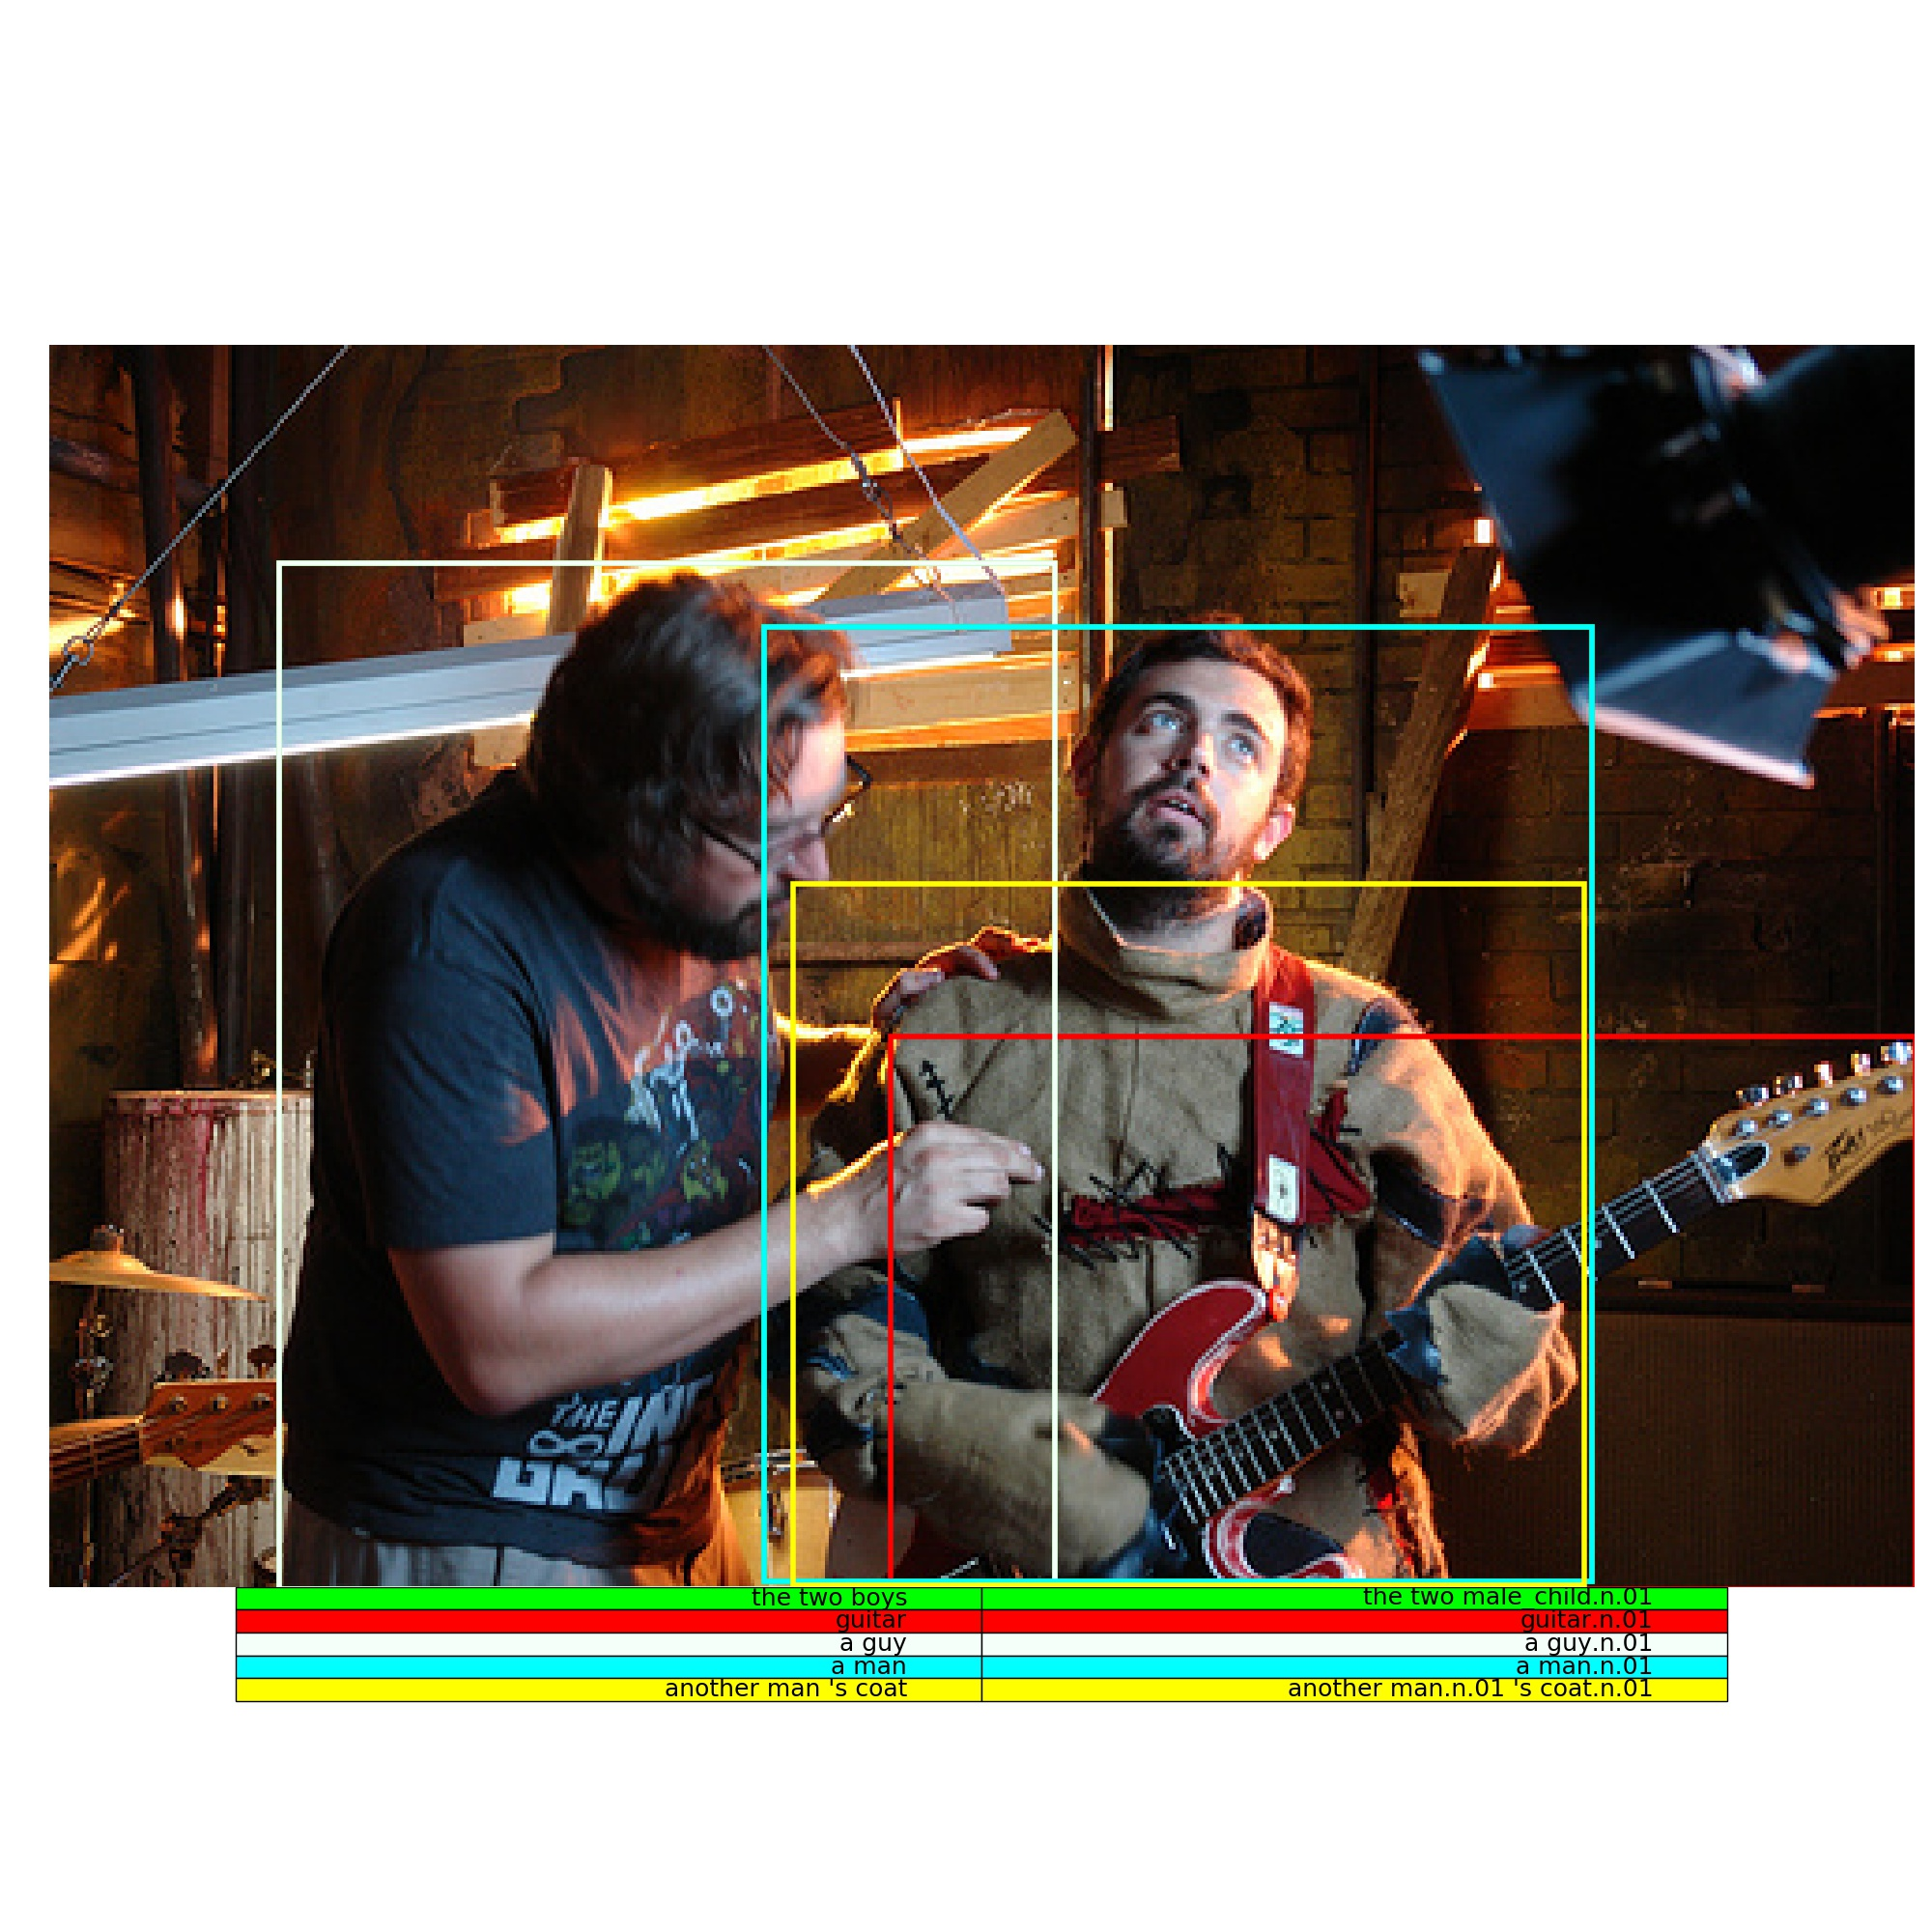
\includegraphics[width=4cm]{fig/flickr_1000523639_boxes.jpg}
		\end{minipage}
		\begin{minipage}{.67\textwidth}	
				{
			\begin{tabular}{l}
				\hline
				\green{[EN$_{39}$ Two people]} in {[EN$_{45}$ the photo]} are playing\\
				\; \red{[EN$_{40}$ the guitar]} and {[EN$_{41}$ the other]} is poking at {[EN$_{0}$ him]} .\\
				
			\blue{[EN$_{42}$ A man]} in \yellow{[EN$_{43}$ green]} holds \red{[EN$_{40}$ a guitar]} while \\
			\;{[EN$_{41}$ the other man]} observes \yellow{[EN$_{43}$ his shirt]} .\\
		
		{[EN$_{41}$ A man]} is fixing \yellow{[EN$_{43}$ the guitar players costume]} .\\
	
	{[EN$_{41}$ a guy]} stitching up \yellow{[EN$_{43}$ another man 's coat]} .\\
	
	\green{[EN$_{39}$ the two boys]} playing \red{[EN$_{40}$ guitar]} \\
	\hline
			\end{tabular}
			}
		\end{minipage}
	
		\caption{Example of \flickr. \label{fig:ex_flickr}}
	\end{center}
\end{figure}



\paragraph{\vgenome}
From a linguistic perspective, object categories (e.g.,~\cat{fawn}, \cat{industrial park}, \cat{opened bag}, \cat{carpet oriental}) are defined pragmatically, and the annotations are rather unstructured. 
For example, as illustrated in Figure~\ref{fig:ex_visualgenome}, the categorization of expressions into one of the three annotation types (region, attributes and relationships), is based on the verbs (\word{is} denotes attributes) and prepositions (\word{at} or \word{in} denotes relationships) \cs{double-check w/ paper}
Note also the spelling mistakes (e.g.,~\word{dalmation}, \word{wating}). 
Furthermore, regions and their annotations are highly redundant in that expressions referring to the same object may still be linked to different bounding boxes\cs{We would need to, e.g., merge boxes through IoU $\geq$ some threshold}. 


As far as object naming is concerned, requirement R1 is not met.    
The annotators were free in their choice of a name for the objects, hence, the latter is usually the entry-level in many annotations. 
For the same reason, on the other hand, and because of the dense image labeling and its exhaustive annotations, \vgenome satisfies R2---we can infer the entry-level name of each object in the image. 
For example, based on frequency estimates, the entry-level for the object on the left is \refexp{dalmatian} (Figure~\ref{fig:ex_visualgenome}), whereas the object on the right is referred to by \refexp{heeler} once, and mostly by \refexp{dog} and its appearance or location. \\


\begin{figure}[t]
	\begin{center}
	\begin{minipage}{.33\textwidth}
		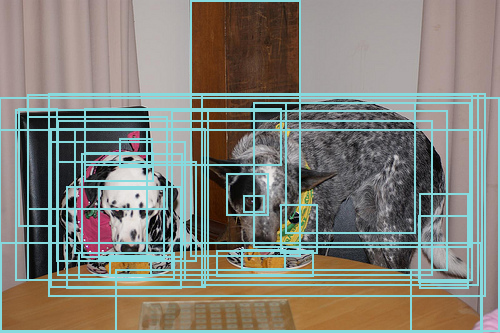
\includegraphics[width=4cm]{fig/visual_genome_dogs.png}
	\end{minipage}
	\begin{minipage}{.65\textwidth}
		\begin{tabular}{l|l}
			\hline
			Annotation	& \\	
			types		& 	\\
			\hline \hline
			Regions &  dalmatian's head; dalmatian dog\\
					& wating at a dinner table; the dog is gray\\
			Attributes & dog is gray; dalmation is eating\\
			Relationships & dog at table; dalmation IN chair; \\
							& heeler eating treat \\
							\hline
		\end{tabular}
	\end{minipage}
	\caption{Example of \vgenome. \label{fig:ex_visualgenome}}
	\end{center}
\end{figure}


\noindent
Finally, requirement~R4 is met by all discussed datasets. 

\cs{XXXXX}\\\\

\subsection{Analysis of Data wrt Our Requirements(?)}

\begin{table}[t]
	\begin{tabular}{lccc}
		\hline
		Resource & \multicolumn{3}{c}{No. categories $cat$ for which $*(cat, \text{ILSVRC})$:} \\
				& $\in$
				& superset
				& $\supset$\\
		\hline \hline
		\refcoco & 15 \\
		\refcocop & \\
		\flickr & \\
		\vgenome & \\
		\hline
	\end{tabular}
	\caption{Coverage of the categories by the $1,000$~synsets of the ILSVRC image classification challenge.  \label{tab:coverage_ilsvrc}}
\end{table}


\subsubsection{Pre-processing}
We parse referring expressions and captions with the Stanford Dependency Parser.
We extract heads/object names as follows: TODO.

\subsubsection{Level of Specificity} 
Variability of reference level in existing data sets for language \& vision?
Are resources appropriate for defining reference level?
\paragraph{WordNet?}

We hypothesize that the distance of a name's synset to the root node (entity) relates to its specificity.
We estimate this distance as the minimal path length of all synsets of a word  to the root node.

Table \ref{tab:specnames} shows the estimated levels of specificity for object names in the RefCoco data set.
We observe distances to the root between 2 and 17, meaning that there is a much more fine-grained distinction of levels than the three-way classification.

Unfortunately, the levels of specificity predicted by WordNet do not seem to reflect linguistic intuitions, here are some problematic examples from Table \ref{tab:specnames}:

\begin{itemize}
\item elephant (10) is more specific than panda (14)? horse is less specific than elephant (10)?
\end{itemize}


\begin{table}
\centering
\setlength{\tabcolsep}{4pt}
\begin{tabular}{rrl}
\toprule
 specificity &  rel.freq. &                          top 5 names \\
\midrule
          -1 &   0.071697 &      NONE,brocolli,zeb,broc,girafe \\
           2 &   0.003898 &                         thing,things \\
           3 &   0.001182 &   object,group,set,substance,objects \\
           4 &   0.140633 &           man,person,piece,head,part \\
           5 &   0.100739 &       player,glass,baby,front,corner \\
           6 &   0.208590 &              woman,girl,kid,boy,bowl \\
           7 &   0.238708 &            guy,right,chair,lady,bear \\
           8 &   0.110613 &           horse,bus,cow,pizza,batter \\
           9 &   0.097390 &         shirt,car,bike,donut,catcher \\
          10 &   0.048368 &   elephant,couch,truck,vase,suitcase \\
          11 &   0.008828 &    motorcycle,clock,mom,dad,scissors \\
          12 &   0.002822 &  oven,airplane,suv,taxi,refrigerator \\
          13 &   0.005253 &   laptop,fridge,canoe,orioles,pigeon \\
          14 &   0.000414 &  panda,freezer,penguin,rooster,rhino \\
          15 &   0.030870 &   zebra,giraffe,zebras,giraffes,deer \\
          16 &   0.000083 &       bison,mooses,orang,elks,sambar \\
          17 &   0.000143 &           ox,cattle,gnu,mustang,orca \\
\bottomrule
\end{tabular}\caption{Levels of specificity for naming choices in RefCOCO: for each level, relative frequency and 5 most frequent names are shown}
\label{tab:specnames}
\end{table}

\paragraph{No. of images in ImageNet?}